%!TEX root = ../../msc17-game-book.tex


\phWorksheet{Solution - Main Puzzle 1}

Since Grendel is equally close to the center of every cauldron used, these centers lay on a big circle with Grendel as the center. The distance to Grendel is minimized by making no gaps between any two cauldrons. As we use fewer and fewer cauldrons the radius of this ``big circle'' is minimized. This means using 3 cauldrons minimizes the distance from Grendel to a cauldron.


\begin{figure}[h!]
\centering
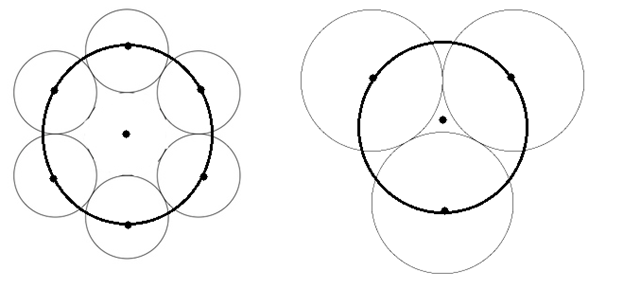
\includegraphics[scale=.5]{assets/josh/circles}
\end{figure}

To determine how close Grendel is in the circle to the right we note the triangle formed by connecting the three circle centers and note Grendel is equally close to them.

\begin{figure}[h!]
\centering
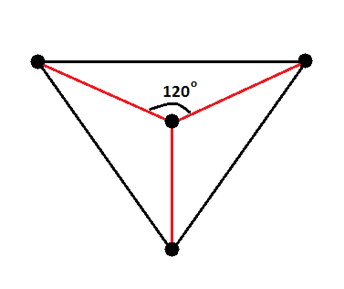
\includegraphics[scale=.5]{assets/josh/bigtri}
\end{figure}

The black lines are equal length and the red lines are equal length so we have 3 equivalent isosceles triangles within an equilateral triangle. So the three angles at the center all equal to one another and sum up to $360^o$. This means each of these angles is $120^o$.

Now let's look at just the ``top two'' circle centers, as well as Grendel.

\begin{figure}[h!]
\centering
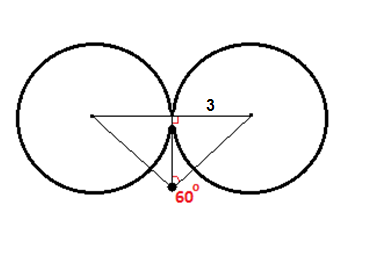
\includegraphics[scale=.5]{assets/josh/circletri}
\end{figure}

By drawing upward from Grendel we will cut the segment between the two circle centers in half. However, what we've really done is form a 30, 60, 90 triangle whose side opposite to the $60^o$ angle is 3. The hypotenuse of this triangle happens to be the distance we are trying to find so all we must do now is use the formula we were given at the start: $y = \frac{2}{\sqrt{3}}x$. (Where y is the hypotenuse and x is the side opposite to the $60^o$ angle)

Plugging is 3 for x yields $y= \frac{6}{\sqrt{3}}=2\sqrt{3}$.
